\documentclass[tikz]{standalone}

\usepackage{tikz}
\usetikzlibrary{automata}

\begin{document}

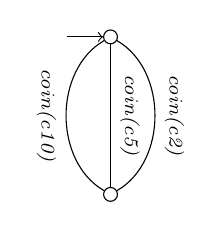
\begin{tikzpicture}
    \tikzstyle{every state}=[
        draw,
        shape=circle,
        inner sep=1pt,
        minimum size=5pt,
        final/.style={double,minimum size=6pt},
        initial text=]

    [auto,->]
    \renewcommand{\a}[1]{\textit{#1}}
    \node[state,initial] (n)  {};
    \node[state] (e) [below of=n, node distance=2cm] {};
    \path
        (n) edge[bend left=60] node[above,rotate=-90]{\scriptsize{\a{coin(c2)}}} (e)
            edge node[above,rotate=-90]{\scriptsize{\a{coin(c5)}}} (e)
            edge[bend right=60] node[below,rotate=-90]{\scriptsize{\a{coin(c10)}}} (e);
\end{tikzpicture}
\end{document}